\begin{columns}[t]
	\begin{column}{0.50\textwidth}
		\begin{block}{\large Motivation}
		    \begin{columns}[t]
			    \begin{column}{0.62\textwidth}
					    If a kinodynamic planner $[1]$ has access to local maneuvers that balance an exploitation-exploration trade-off, the planner's per iteration performance is significantly improved.
					    \begin{itemize}
					    	\item Exploitation maneuvers guide the system towards the goal given local heuristic information
					    	\item Exploration maneuvers move the system in different directions so as to deal with situations that the heuristic does not provide good guidance.
					    \end{itemize}
					    % \item These maneuvers can be computed online employing a metric similar to $[2]$, tailored to each state of the robot selected for propagation during planning.
			    \end{column}
			    \begin{column}{0.35\textwidth}
			    	\centering
					\begin{figure}
					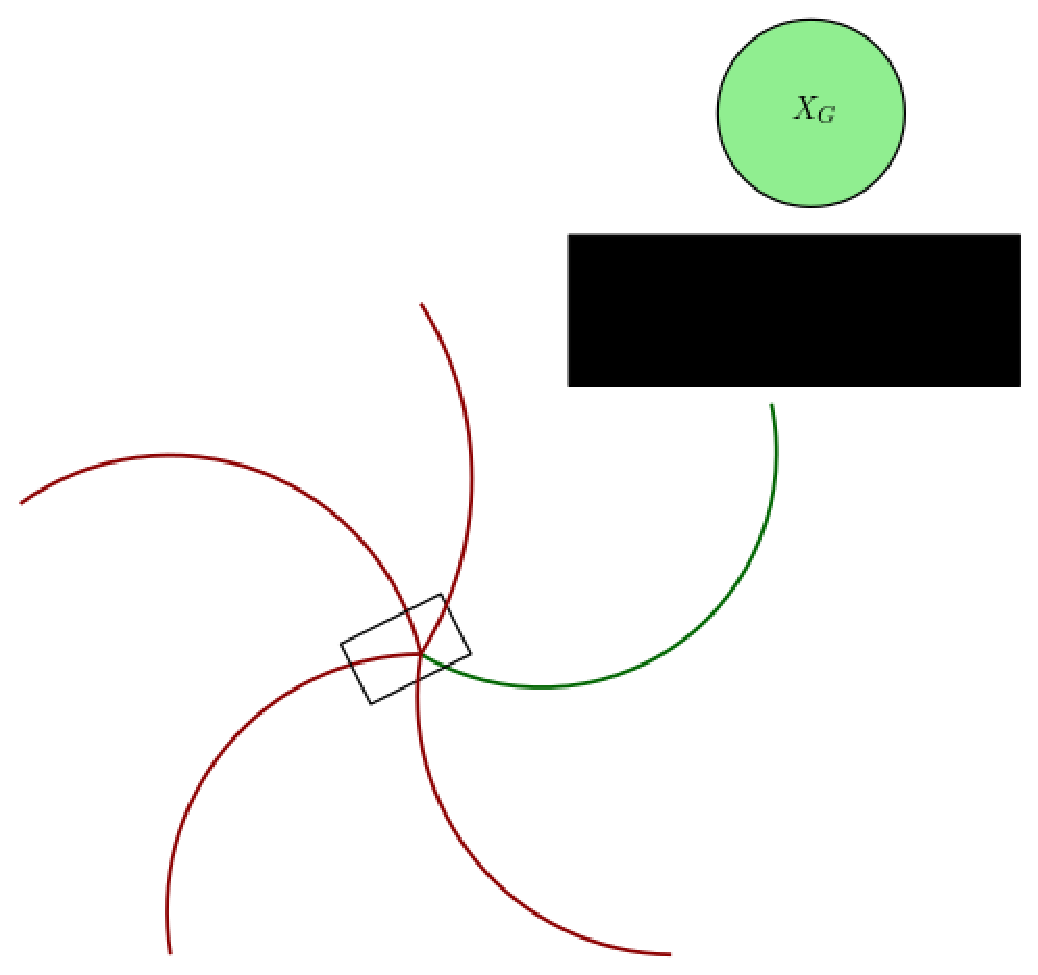
\includegraphics[scale=0.67]{figures/maneuver_sets.eps}
					\caption{Exploitative (green) and Explorative (red) maneuvers for a robot planning to reach $X_G$ (green circle) behind an obstacle (black box). \vspace{-.2in}}
					\end{figure}
			    \end{column}
		    \end{columns}
		\end{block}
	\end{column}
	\begin{column}{0.50\textwidth}
		\begin{block}{\large Motion planning with informed maneuvers}
		    % \centering
		    % 	\begin{figure}[h]
		    % 		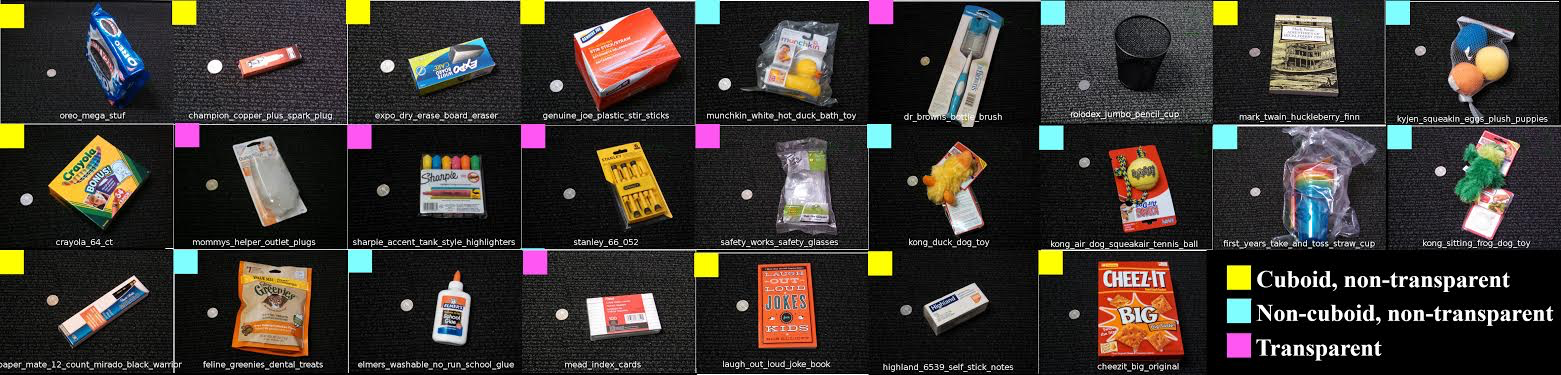
\includegraphics[width = 0.75\textwidth, height=2.5in]{meta_items}	\hspace{0.1in}
		    % 		\caption{The 25 APC objects categorized by broad object class}
	    	% 	\end{figure}
	    	% 	\vspace{-0.2in}
		    \begin{columns}[T]
		    	\begin{column}{0.98\textwidth}
					\begin{itemize}
						\item Informed maneuvers can be computed online employing a metric similar to $[2]$, tailored to each state of the robot selected for propagation during planning. \vspace{0.1in}
						\begin{table}[h!]
						\centering
						\begin{tabular}{|l|l|l|l|}
						\hline
						        & \textbf{Iteration} & \textbf{Comp. Time} & \textbf{Path Cost} \\ [0.5ex] \hline
						Random  & 1471                    & 0.2                   & 50.47                  \\ \hline
						Curated & 686                    & 12.15                & 48.13                  \\ \hline
						\end{tabular}
						\caption{First solution statistics between DIRT using random and curated maneuvers.}
						\label{table:Rastar}
						\vspace{0.1in}
					\end{table}
						\item Very effective in finding a high-quality solution in fewer number of iterations but computational becomes prohibitive.
						\item \textbf{Goal:} Develop an approach that achieves the same objective as the curation but can generate the maneuvers fast.
					\end{itemize}
				\end{column}
				% \begin{column}{0.38\textwidth}
				% 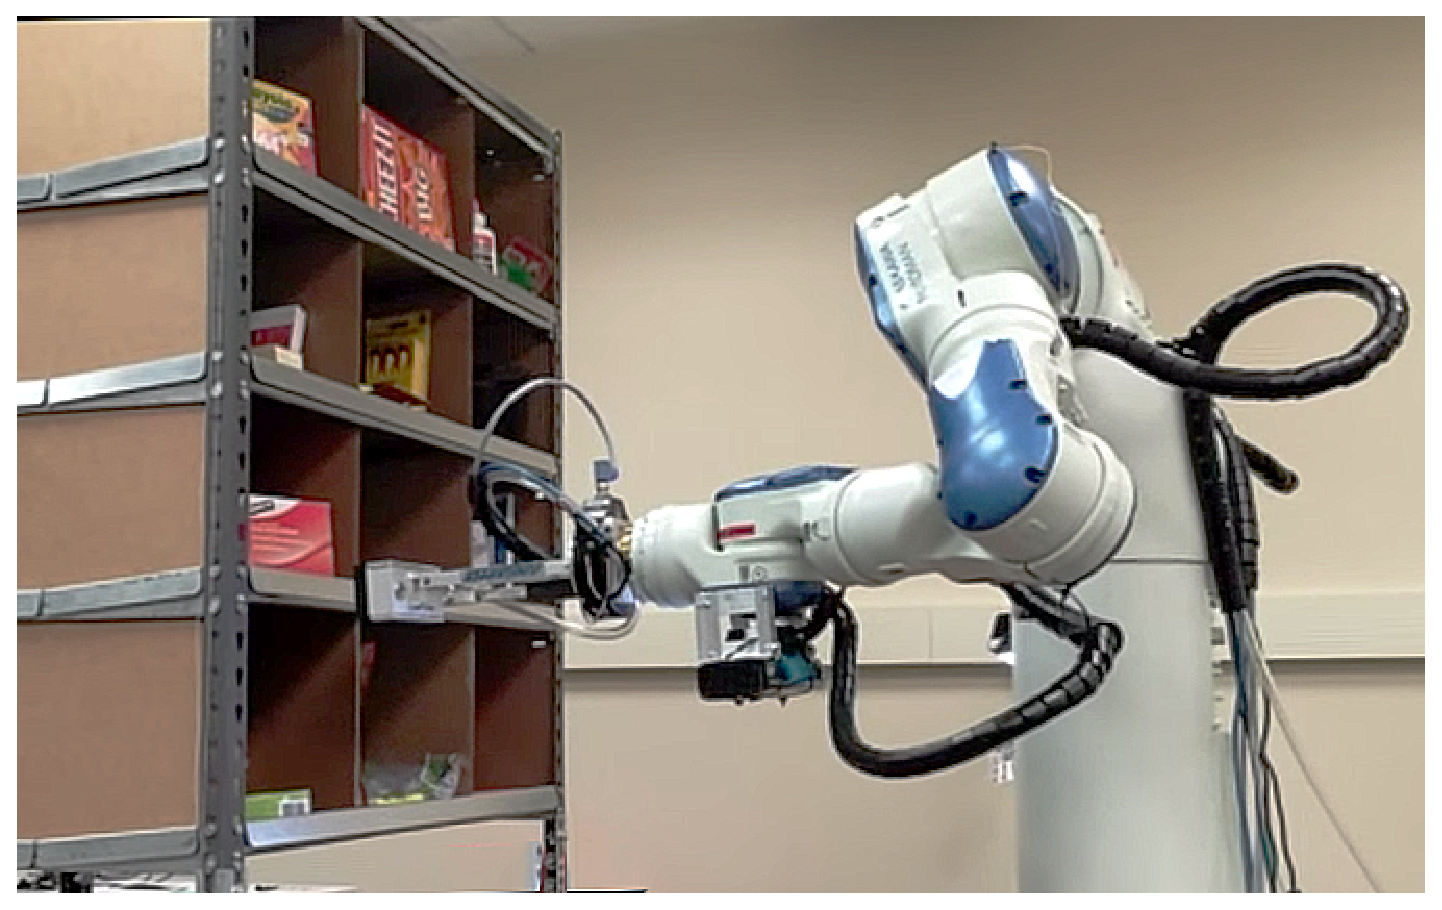
\includegraphics[height=2.5in]{datacollectionsetup_2}	\hspace{0.1in}
				% \end{column}
			\end{columns}
		\end{block}
	\end{column}
\end{columns}	
		    
